\documentclass[preprint,12pt]{elsarticle}

\usepackage{amsmath,amssymb,amsfonts}
\usepackage{algorithmic}
\usepackage{graphicx}
\usepackage{textcomp}
\usepackage{xcolor}
\usepackage{booktabs}
\usepackage{multirow}
\usepackage{url}
\usepackage{array}
\usepackage{lineno}
\usepackage{hyperref}
\usepackage{tikz}
\usetikzlibrary{positioning,arrows.meta}

\journal{Journal of Systems and Software}

\begin{document}

\linenumbers

\title{Design Mining in Software Projects Using Transformer Models: A Cross-Project Evaluation on JIRA Tickets}

\author[binghamton]{Steven Morgan}
\author[umgc]{Jeff Daniels, Ph.D.}
\affiliation[binghamton]{organization={Department of Systems Science and Industrial Engineering, Binghamton University, State University of New York},
            city={Binghamton},
            state={NY},
            postcode={13902},
            country={USA}}
\affiliation[umgc]{organization={Graduate School of Technology, University of Maryland Global Campus},
            city={Adelphi},
            state={MD},
            postcode={20783},
            country={USA}}


\begin{frontmatter}
\begin{abstract}
Architectural design work in software projects is widely acknowledged as critical to project success, yet detecting and quantifying such work remains challenging. This paper investigates whether transformer based models can outperform existing techniques for design mining,  the automated classification of design related discussions in software engineering artifacts. We fine tune three transformer architectures (BERT, RoBERTa, and DistilBERT) on the Stack Overflow design mining dataset of Mahadi et al. and then transfer the resulting classifiers to 1,786 manually labeled JIRA issues drawn from ten projects in the TAWOS (Tawosi Agile Web hosted Open Source) dataset. A hyperparameter search across ten configurations yields a best F1 of 0.907 and ROC AUC of 0.965 on the Stack Overflow benchmark. For cross project generalization on TAWOS, leave one project out (LOPO) evaluation with metadata enrichment and square root softened inverse frequency class weighting achieves a mean F1 of 0.733 ($\sigma$ = 0.10), exceeding feature matched support vector machine (F1 = 0.666) and gradient boosting (F1 = 0.636) baselines, though the per project gap is heterogeneous and not significant on every project under a Wilcoxon signed-rank test. Integrated gradients attribution analysis shows the model attends to plausibly design related vocabulary but also to project specific terms (Docker, Helm, plug-in) that explain much of the cross project variance. We discuss the implications of an inherent recall bias under TAWOS’s 28\% design prevalence for downstream tooling and outline the limitations of using single annotator labels and keyword derived pseudo labels as ground truth.
\end{abstract}

\begin{keyword}
Design mining, software architecture, transformer models, BERT, text classification, JIRA, cross-project generalization, transfer learning
\end{keyword}

\end{frontmatter}

\section{Introduction}

There is a fundamental gap between how information technology systems are designed and how they are implemented. Critical requirements can be entirely misconstrued, leaving users to manage workarounds. Project Management, Enterprise Architecture, Systems Architecture, and Systems Engineering have all been applied to varying degrees to implement technical solutions, yet they consistently fall short of meeting project expectations. Project success is typically defined as finishing on time, on budget, and meeting predefined scope~\cite{loureiro2024}.

The Standish Group's CHAOS report, based on surveys of approximately 5,000 software projects annually, found that between 2010 and 2015, only 36\%--41\% of software projects were considered successful, with roughly 20\% classified as outright failures~\cite{standish2015}. As of 2024, worldwide IT spending was expected to exceed \$5 trillion~\cite{gartner2024}. These figures underscore the magnitude of waste that can be attributed to poor project outcomes.

Agile project implementations and smaller projects tend to exhibit higher success rates. The CHAOS Report indicates that Agile teams are up to four times more effective at delivering projects. Meanwhile, 58\% of small projects with clear goals and objectives tend to succeed~\cite{sandle2020}. Agile methodologies emphasize that software differs from traditional engineering because detailed upfront designs can quickly become irrelevant in dynamic environments. Pereira et al.~\cite{pereira2021} developed an evaluation technique to assess project success through the perspectives of practitioners, finding that 36\% of practitioners considered their projects to only partially succeed or fail.

Soft Computing offers a variety of techniques for analyzing systems behavior, including neural networks, evolutionary computing, fuzzy logic, and agent-based modeling. There has been some success in applying these methods to predict faults in software, identify changes in team velocity, and automatically categorize issues~\cite{afzal2011, mahdi2021, pospieszny2018, petkovic2016, zhang2003}. Nature-inspired optimization algorithms and neural networks are among the most common approaches~\cite{mahajan2022, siva2023a, sarro2021, siva2023b}.

Despite these advances, there is a lack of clarity between accepted methods for identifying architectural work in software programs and understanding its impact on project outcomes. Research to automate and classify design-related work, referred to as \emph{design mining}, has been carried out using traditional soft computing techniques~\cite{mahadi2021}. Preliminary research has employed transformers for help desk support and defect prediction~\cite{incekas2024, zangari2023}, yet little work has examined whether transformers (or automation in general) can improve our understanding of architectural work and its relationship to project success, which is the underlying motivation of this research.

This paper addresses the first of three interconnected research questions from a larger investigation: \emph{Can design mining be performed on tickets collected from JIRA using transformers to outperform the state-of-the-art?} This question is valuable because little research of this nature has been performed specific to software engineering tickets. TAWOS contains over 458,000 issues and 1.6 million comments from 39 open-source projects. By demonstrating improved detection of design work at scale, subsequent research can investigate whether such detection predicts changes in defect rates and whether the temporal distribution of architectural effort influences project quality.

The contributions of this paper are:
\begin{enumerate}
\item Application of design mining to the TAWOS dataset, representing operational viability for design mining in practical settings.
\item A comprehensive cross-project generalization analysis using leave-one-project-out validation, demonstrating that transformer models outperform traditional machine learning baselines.
\item Attribution analysis using integrated gradients to explain classification decisions and identify challenges for cross-project generalization.
\end{enumerate}

\section{Related Work}

\subsection{Machine Learning in Software Engineering}

Machine learning has been extensively applied to software engineering problems including defect prediction, effort estimation, and bug triaging. Afzal and Torkar~\cite{afzal2011} performed a systematic literature review of genetic programming applied to software projects, finding it performed comparably to neural networks and logistic regression for project estimation, while outperforming other techniques for fault tolerance and quality prediction.

Software fault prediction has been studied using a variety of techniques. Vineeta and Srinivasan~\cite{vineeta2019} used random forests and Na\"ive Bayes on the NASA Promise dataset, finding both achieved greater than 90\% accuracy. Siva et al.~\cite{siva2023a} applied adaptive artificial jelly optimization with LSTM to achieve 93\% accuracy for bug prediction.  Siva et al.~\cite{siva2023b} later introduced an adaptive golden eagle optimizer for feature selection, achieving 80\% accuracy on PROMISE data and 85\% on NASA data. Mahajan and Chaudhary~\cite{mahajan2022} achieved 85.1\% improvement over the state of the art for bug localization using a cuckoo search-based optimization with CNN.

Estimating software development costs remains one of the primary reasons projects fail to sustain funding. Pospieszny et al.~\cite{pospieszny2018} compared support vector machines, multi-layer perceptrons, and generalized linear models, finding all methods appropriate for predicting software estimates, with the support vector machine performing best at predicting cost and duration. The TAWOS dataset has been used for effort estimation by Tawosi et al.~\cite{tawosi2022}, though neither their deep learning approach nor the TF-IDF baseline of Choetkiertikul et al.~\cite{choetkiertikul2019} proved effective at estimating issue completion across most projects.

\subsection{Design Mining}

Design mining is the automated identification of design-related discussions in software engineering artifacts. It was advanced significantly by Mahadi et al.~\cite{mahadi2021}. Their approach introduced pre-labeled Stack Overflow data and demonstrated applicability to GitHub projects using a back-propagation network, outperforming ten alternative algorithms. Their key contributions included reducing the need for human-labeled data and developing a software-specific vocabulary extracted from academic papers.

Kleebaum et al.~\cite{kleebaum2021} developed ConDec, a tool that plugs into JIRA to elicit decision records, using logistic regression with high recall but poor precision. Mouna Dhaouadi et al.~\cite{dhaouadi2023} extracted decision rationale from Linux commit messages using gradient boosting with TF-IDF features. Sebastian et al.~\cite{sebastian2020} proposed a machine learning pipeline for detecting software architecture degradation, though their systematic review found little prior research combining detection with causal analysis and remediation.

Moore et al.~\cite{moore2003} attempted to quantify architecture effort using qualitative measures such as stakeholder quality, while Nord et al.~\cite{nord2014} reviewed approaches for capturing design quality metrics, all involving qualitative scoring. These approaches require direct human involvement for consistent information capture, motivating the need for automated methods.

\subsection{Defect Prediction and Feature Selection}

Li et al.~\cite{li2024} surveyed software defect prediction, identifying key future directions including data labeling quality, deep learning models, privacy-preserving data sharing, multi-feature fusion, line-level prediction, and unsupervised learning. Matloob et al.~\cite{matloob2021} found random forest, boosting, and bagging to be the most common ensemble methods, with AUC, accuracy, and recall as the most common performance measures. Giray et al.~\cite{giray2023} found that CNNs and RNNs were the most commonly used deep learning approaches, noting external features such as documentation or tickets are seldom used for prediction.

Ali et al.~\cite{ali2023} performed a systematic review of feature selection methods, categorizing them as filter, wrapper, embedded, and hybrid, with filter and hybrid being most common. Li et al.~\cite{li2023} demonstrated that XGBoost performed best for feature identification when compared across nine classifiers for effort-aware defect prediction.

Liu et al.~\cite{liu2023} showed that using code comments and commit messages as external knowledge improved defect detection over code-only features. Wang et al.~\cite{wang2024} demonstrated improved accuracy for bug triaging using Bi-LSTM with attention and ELMo across 35 models.

\subsection{Transformer Models for Text Classification}

BERT (Bidirectional Encoder Representations from Transformers)~\cite{devlin2019} provides contextual awareness by processing text bidirectionally, making it well-suited for classification tasks. BERT can be fine-tuned with small datasets and requires modification of only a single classification layer. It builds upon ELMo~\cite{peters2018} and GPT~\cite{radford2018}, combining bidirectional context with simplified fine-tuning.

Trust and Minghim~\cite{trust2024} compared eight large language models using various fine-tuning techniques, finding BERT variants performed best on classification tasks. Mullis et al.~\cite{mullis2023} demonstrated above 90\% accuracy when using BERT to classify functional and non-functional requirements in engineering documents. Yucalar~\cite{yucalar2023} achieved a 95\% F-score using BERT on Turkish software requirements, confirming cross-language effectiveness. Nursapa et al.~\cite{nursapa2025} compared CodeBERT and CodeT5 for architectural smell detection, with CodeT5 consistently outperforming CodeBERT while both maintained at least 80\% effectiveness.

Zhang and Wu~\cite{zhang2020} used abstract syntax trees combined with transformer-based word embeddings, achieving 8\% improvement over other deep learning approaches for defect prediction. Incekas~\cite{incekas2024} found BERTopic highly effective for topic modeling of help desk tickets. However, Zangari et al.~\cite{zangari2023} found that traditional SVM outperformed BERT for multi-level ticket classification, attributing this to noisy underlying datasets.

\section{Research Method}

\subsection{Overview}

This research employs a quantitative, experimental design using transformer-based machine learning to determine whether design mining can be performed on JIRA tickets to outperform the current state-of-the-art. The approach follows a sequential methodology: (1)~fine-tune transformer models on labeled Stack Overflow data, (2)~apply transfer learning and manual labeling to the TAWOS dataset, and (3)~compare transformer performance against traditional machine learning baselines using cross-project validation. Figure~\ref{fig:pipeline} summarizes this pipeline.

In this paper, \emph{design mining} refers specifically to the binary text classification of individual JIRA tickets as design-related or not, following the terminology and task framing of Mahadi et al.~\cite{mahadi2021}; it does not extract design artifacts, decisions, or architectural models from those tickets. Section~\ref{sec:discussion} returns to this scoping when discussing downstream applications.

\begin{figure}[t]
\centering
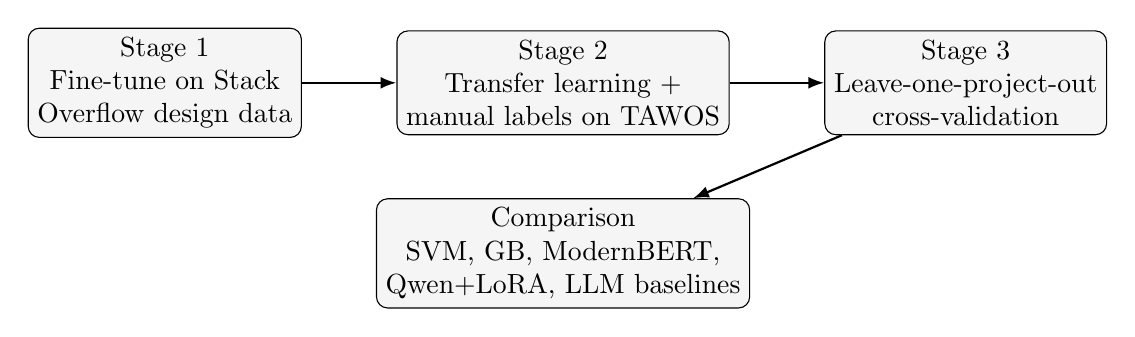
\begin{tikzpicture}[
  node distance=8mm and 12mm,
  stage/.style={rectangle, draw, rounded corners, align=center, minimum width=3.1cm, minimum height=1.1cm, fill=gray!8},
  arr/.style={-{Latex[length=2mm]}, thick}
]
\node[stage] (so) {Stage 1\\Fine-tune on Stack\\Overflow design data};
\node[stage, right=of so] (transfer) {Stage 2\\Transfer learning +\\manual labels on TAWOS};
\node[stage, right=of transfer] (lopo) {Stage 3\\Leave-one-project-out\\cross-validation};
\node[stage, below=of transfer] (compare) {Comparison\\SVM, GB, ModernBERT,\\Qwen+LoRA, LLM baselines};
\draw[arr] (so) -- (transfer);
\draw[arr] (transfer) -- (lopo);
\draw[arr] (lopo) -- (compare);
\end{tikzpicture}
\caption{Overview of the three-stage pipeline: Stack Overflow pretraining, TAWOS transfer learning with manual and cherry-picked labels, and leave-one-project-out cross-validation against traditional-ML, modern-encoder, and LLM baselines.}
\label{fig:pipeline}
\end{figure}

\subsection{Datasets}

Two primary datasets are used. The \textbf{Stack Overflow Design Mining Dataset}~\cite{mahadi2021} contains approximately 260,000 labeled discussions from Stack Overflow, pre-processed and vectorized for software engineering text. Labels are binary: \emph{design} or \emph{non-design}. The dataset includes software-specific stop words and two vectorization techniques (TF-IDF and word embeddings).

The \textbf{TAWOS Dataset}~\cite{tawosi2022} contains 458,232 issues from 39 open-source projects collected from JIRA repositories. Unlike Stack Overflow, TAWOS issues represent planned work with effort information, relationships to other issues, descriptions, and comments, providing richer context for design mining at an operational level.

\subsection{Data Preprocessing}

For the Stack Overflow dataset, existing preprocessing and vectorization from Mahadi et al.~\cite{mahadi2021} was derived based on the available dataset and literature. For the TAWOS dataset, preprocessing included removing duplicate issues, filtering automatically generated issues, normalizing whitespace, and removing URLs, email addresses, and system-generated information. The same software-specific stop words based on the Mahadi dataset were applied for consistency when comparing methods, however, it was found that the stop words caused degraded performance with transformer models.

\subsection{Labeling the TAWOS Dataset}

Initial transfer learning using the Stack Overflow fine-tuned model exhibited self-affirmation bias, producing near-perfect but invalid scores. To address this, 1,786 issues from ten projects were manually reviewed and labeled. Projects were selected across different repositories to ensure variety and reduce bias.

During manual review, design issues were defined as those involving documentation or creation of architecture, code or process refactoring for project-level improvement, or design for new features. Non-design issues included bug fixes, code cleanup, and implementation tasks with clear scope. Of the manually labeled issues, 28\% were classified as design, a significant class imbalance compared to the 50/50 split in the Stack Overflow data.

To address this imbalance, a cherry-picking heuristic was developed to identify high-probability design examples. Issues were first passed through a set of hard exclusion rules: issue type (bug, sub-task, test task, technical task), version-upgrade or migration language, documentation-only changes, issues containing Java stack traces or requests for improved logging, any mention of deployment, and summaries dominated by UI-only vocabulary (e.g. \emph{button}, \emph{css}, \emph{tooltip}). Surviving issues were then scored using a weighted keyword lexicon searched over the issue summary and description: 37 strong architectural phrases (e.g. \emph{microservices}, \emph{event-driven}, \emph{api gateway}, \emph{oauth}, \emph{message broker}) contributed $+3$ points each, 31 medium-signal phrases (e.g. \emph{refactor}, \emph{authentication}, \emph{caching}, \emph{rate limit}) contributed $+2$, and 10 weak, single-word signals (e.g. \emph{api}, \emph{service}, \emph{plugin}) contributed $+1$; issue type also carried a bonus of $+2$ or $+3$ for feature/enhancement/story-type issues. Small, cosmetic API changes and single UI-signal words were penalized at $-2$ each. A minimum total of 5 points was required for selection, yielding 415--4,890 design labels per source (5,021 design / 1,290 non-design in total; Table~\ref{tab:labels}) depending on whether the source was a curated project export (top-35-per-file plus 100 cross-file candidates) or an unfiltered TAWOS database pull (all issues scoring above threshold). A manual audit of 100 sampled heuristic labels found approximately 95\% agreement with a human reviewer (5 disagreements).

The heuristic's own volume is itself a source of the noise it introduces: Table~\ref{tab:lopo} shows that LOPO performance improves as up to 250 cherry-picked design examples are added to the 1,786 manually labeled tickets (mean F1 rising from 0.711 to 0.719), but degrades monotonically beyond that (falling to 0.695 when all $\sim$10K cherry-picked labels are used), which we interpret as the heuristic's precision degrading once the highest-confidence, highest-scoring candidates are exhausted and lower-scoring, noisier tickets are admitted.

\begin{table}[t]
\centering
\caption{Final Label Count for Fine-Tuning on TAWOS Data}
\label{tab:labels}
\begin{tabular}{lcc}
\toprule
\textbf{Source} & \textbf{Design} & \textbf{Non-Design} \\
\midrule
Manually Labeled & 478 & 1,290 \\
Cherry-Picked & 4,890 & 4,995 \\
\midrule
\textbf{Total} & \textbf{5,368} & \textbf{6,285} \\
\bottomrule
\end{tabular}
\end{table}

\subsection{Evaluation Metrics}

Following Mahadi et al.~\cite{mahadi2021}, accuracy and AUC are used as metrics, supplemented by precision and recall. The F1 score is considered the primary metric because it is best used to measure the accuracy of an unbalanced dataset. Accuracy is defined as:
\begin{equation}
\text{Acc} = \frac{TP + TN}{TP + TN + FP + FN}
\label{eq:acc}
\end{equation}
Recall measures correctly identified positives:
\begin{equation}
\text{Recall} = \frac{TP}{TP + FN}
\label{eq:recall}
\end{equation}
Precision measures the ratio of true positives among all positive classifications:
\begin{equation}
\text{Prec} = \frac{TP}{TP + FP}
\label{eq:prec}
\end{equation}
The F1 score is the harmonic mean of precision and recall:
\begin{equation}
F_1 = \frac{2 \cdot \text{Prec} \cdot \text{Recall}}{\text{Prec} + \text{Recall}}
\label{eq:f1}
\end{equation}
AUC is calculated as:
\begin{equation}
\text{AUC} = \frac{\frac{TP}{TP+FN} + \frac{TN}{TN+FP}}{2}
\label{eq:auc}
\end{equation}

\subsection{Model Architecture}

The BERT base model uses a 512-token limit with a BERT tokenizer. Each example receives a \texttt{[CLS]} token denoting the instance and \texttt{[SEP]} tokens marking separations between fields. For example: \texttt{[CLS] Document reasoning for using event-driven architecture [SEP] Create an architecture decision record [SEP]}. Each token embedding combines word embedding, segment embedding, and position embedding.

Fine-tuning adds a classification layer on top of the pre-trained model. An initial fine-tuning stage uses the Stack Overflow dataset with a learning rate of 2e-5, batch size of 16, and 3--5 epochs. A second fine-tuning stage uses the TAWOS labeled data with a smaller learning rate and fewer epochs for more modest adaptation. A dropout layer prevents overfitting, and a dense layer with Softmax provides classification probabilities.

\subsection{Comparison with Traditional Methods}

To provide a fair baseline, support vector machine (SVM) and gradient boosting (GB) models were trained using hyperparameter grid search with stratified 5-fold cross-validation. For SVM, 12 combinations were tested over regularization strength ($C \in \{0.1, 1, 10\}$), kernel (RBF, linear), and gamma (scale, auto). For GB, 54 combinations were tested over number of estimators ($\{100, 200, 300\}$), max depth ($\{3, 5, 7\}$), learning rate ($\{0.01, 0.1, 0.2\}$), and subsample ($\{0.8, 1.0\}$). With 5-fold validation, this resulted in 330 model combinations tested.

\section{Results}

\subsection{Stage 1: Fine-Tuning on Stack Overflow Data}

Ten experiments were completed across \texttt{bert-base-uncased}, \texttt{roberta-base}, and \texttt{distilbert-base-uncased} using the Mahadi et al.~\cite{mahadi2021} Stack Overflow dataset with the same training and validation splits. Results are shown in Table~\ref{tab:stage1}.

\texttt{roberta-base} with a conservative learning rate of 1e-5 achieved the best F1 score of 0.9066 and AUC of 0.9650. \texttt{bert-base-uncased} was a close second (F1=0.9056, AUC=0.9646). All models performed similarly, with aggressive learning rates causing rapid overfitting (F1 $\approx$ 0.5).

\begin{table}[t]
\centering
\caption{Stage 1 Results: Training on Stack Overflow Data}
\label{tab:stage1}
\begin{tabular}{lccccc}
\toprule
\textbf{Model} & \textbf{BS} & \textbf{LR} & \textbf{E} & \textbf{F1} & \textbf{AUC} \\
\midrule
roberta & 16 & 1e-5 & 3 & \textbf{0.907} & 0.965 \\
roberta & 32 & 2e-5 & 3 & 0.907 & \textbf{0.966} \\
roberta & 16 & 2e-5 & 3 & 0.906 & 0.965 \\
roberta & 16 & 5e-6 & 5 & 0.905 & 0.965 \\
bert & 32 & 2e-5 & 3 & 0.906 & 0.965 \\
distilbert & 32 & 2e-5 & 3 & 0.906 & 0.964 \\
distilbert & 16 & 2e-5 & 3 & 0.905 & 0.964 \\
distilbert & 16 & 1e-5 & 3 & 0.905 & 0.964 \\
bert & 16 & 5e-6 & 5 & 0.905 & 0.963 \\
distilbert & 16 & 5e-6 & 5 & 0.905 & 0.963 \\
\bottomrule
\end{tabular}
\begin{flushleft}
\footnotesize BS = Batch Size, LR = Learning Rate, E = Epochs
\end{flushleft}
\end{table}

\subsection{Stage 2: Transfer Learning to TAWOS}

Transfer learning experiments used RoBERTa and BERT fine-tuned first on Stack Overflow data, then adapted to the TAWOS dataset. Transfer learning in this context is an attempt to label data based on the Stack Overflow fine tuned model. The data labeled by the fine tuned model was then used to adapt the model according to the TAWOS dataset. A 60/20/20 training/test/evaluation split was used. Inverse-frequency class weights on cross-entropy loss~\cite{mao2023} addressed the class imbalance. Results are shown in Table~\ref{tab:transfer}. The purpose of attempting transfer learning was to address the small number of manually labeled data, the cherry-picking method was an attempt to address the overly optimistic results of transfer learning.

The \texttt{roberta\_transfer} configuration using inverse-frequency class weighting achieved an F1 of 0.9597, while the balanced configuration (\texttt{roberta\_transfer\_balanced}) reached F1 of 0.9804. However, the near-perfect results for all models suggested that transfer learning was overfitting data and creating confirmation bias in the training. Effectively, the models had learned how each fine-tuned version would label and classify, hence re-affirming itself.

\begin{table}[t]
\centering
\caption{Transfer Learning Validation Metrics (Best Epoch)}
\label{tab:transfer}
\begin{tabular}{lcccc}
\toprule
\textbf{Experiment} & \textbf{Prec} & \textbf{Rec} & \textbf{F1} & \textbf{AUC} \\
\midrule
roberta\_transfer & 0.948 & 0.972 & 0.960 & 0.979 \\
roberta\_balanced & \textbf{0.966} & \textbf{0.995} & \textbf{0.980} & 0.947 \\
bert\_conservative & 0.915 & 0.921 & 0.918 & \textbf{0.994} \\
\bottomrule
\end{tabular}
\end{table}

\subsection{Cross-Project Generalization (LOPO)}

Leave-one-project-out (LOPO) analysis trained on nine projects and validated on the held-out project. Various configurations of data augmentation, layer freezing, and manual weighting were tested. Table~\ref{tab:lopo} presents the aggregated results.

The \texttt{Aug top-250} configuration, augmenting with 250 balanced cherry-picked samples, achieved the best mean F1 of 0.7189. The baseline with only manual labels achieved F1=0.7111 with the best AUC of 0.8983 and lowest variance. Additional augmentation beyond 250 samples showed monotonically decreasing performance, contradicting prior studies~\cite{nam2013, uddin2022} that found augmentation improved results.

The freezing of layers 10 substantially degraded the results (F1=0.6188 for manual-only), although combining the freezing with the full augmented data set partially recovered the performance (F1 = 0.6535). Pseudo-labels from Stack Overflow transfer learning also underperformed the baseline.

\begin{table}[t]
\centering
\caption{LOPO Cross-Validation Results (RoBERTa)}
\label{tab:lopo}
\setlength{\tabcolsep}{3pt}
\begin{tabular}{lccccc}
\toprule
\textbf{Config} & \textbf{Aug} & \textbf{$\bar{F_1}$} & \textbf{$\sigma_{F_1}$} & \textbf{$\bar{\text{AUC}}$} & \textbf{$\bar{\text{Acc}}$} \\
\midrule
Aug-250 & 500 & \textbf{0.719} & 0.100 & 0.893 & \textbf{0.819} \\
Aug-500 & 1000 & 0.713 & 0.084 & 0.896 & 0.816 \\
Baseline & 0 & 0.711 & \textbf{0.076} & \textbf{0.898} & 0.813 \\
Aug-750 & 1500 & 0.700 & 0.105 & 0.880 & 0.805 \\
Aug all & $\sim$10K & 0.695 & 0.095 & 0.886 & 0.811 \\
Aug-1000 & 2000 & 0.689 & 0.112 & 0.874 & 0.793 \\
Freeze 10+aug & $\sim$10K & 0.654 & 0.114 & 0.861 & 0.748 \\
Freeze 10 & 0 & 0.619 & 0.087 & 0.837 & 0.732 \\
\bottomrule
\end{tabular}
\begin{flushleft}
\footnotesize Aug = total augmented samples (design + non-design)
\end{flushleft}
\end{table}

The model exhibited a recall bias with weaker precision, indicating a tendency to over-label issues as design (mean recall 0.814 vs. mean precision 0.634 for Aug-250). Certain projects consistently scored lower: SERVER and DM both achieved F1=0.59, while CONFSERVER reached 0.83 on the baseline. The design rate within a project's sample did not correlate with performance, DNN scored F1=0.79 with 25\% design rate, whereas SERVER scored 0.48 with 20\%. This suggests that project-specific language variation, rather than class balance, is the primary challenge.

\subsection{Comparison with SVM and Gradient Boosting}

The best cross-validated configuration for GB used a learning rate of 0.2, max depth of 3, 100 estimators, and subsample of 1.0 (F1=0.753). The best SVM used $C$=1, linear kernel, and gamma=scale (F1=0.721).

LOPO analysis with these optimized configurations (Table~\ref{tab:lopo_trad}) shows that SVM performed best without augmentation (F1=0.666, AUC=0.861), while GB benefited from augmentation (F1=0.636, AUC=0.841). RoBERTa's best LOPO result (F1=0.719) outperformed both SVM ($+$7.9\%) and GB ($+$13.1\%).

\begin{table}[t]
\centering
\caption{LOPO Analysis: SVM and Gradient Boosting}
\label{tab:lopo_trad}
\setlength{\tabcolsep}{3pt}
\begin{tabular}{llccccc}
\toprule
\textbf{Config} & \textbf{Model} & \textbf{$\bar{F_1}$} & \textbf{$\bar{\text{AUC}}$} & \textbf{$\bar{\text{Acc}}$} & \textbf{$\bar{\text{Prec}}$} & \textbf{$\bar{\text{Rec}}$} \\
\midrule
Baseline & SVM & \textbf{0.666} & \textbf{0.861} & \textbf{0.810} & \textbf{0.652} & 0.699 \\
Baseline & GB & 0.604 & 0.823 & 0.780 & 0.592 & 0.630 \\
Aug-250 & SVM & 0.658 & 0.852 & 0.784 & 0.590 & 0.759 \\
Aug-250 & GB & 0.633 & 0.832 & 0.779 & 0.583 & 0.704 \\
Aug-500 & SVM & 0.660 & 0.855 & 0.774 & 0.576 & \textbf{0.797} \\
Aug-500 & GB & 0.636 & 0.841 & 0.772 & 0.574 & 0.723 \\
\bottomrule
\end{tabular}
\end{table}

\subsection{Metadata Enrichment and Weighting Optimization}

Adding JIRA issue type and priority as additional \texttt{[SEP]}-delimited fields, combined with a softened class weighting strategy, further improved results (Table~\ref{tab:meta}). The softened weighting applied a square root to the inverse-frequency weights:
\begin{subequations}\label{eq:weights}
\begin{align}
w_{\text{neg}} &= \sqrt{\text{total} \mathbin{/} (2 \cdot n_{\text{neg}}) \label{eq:wneg}} \\
w_{\text{pos}} &= \sqrt{\text{total} \mathbin{/} (2 \cdot n_{\text{pos}}) \label{eq:wpos}}
\end{align}
\end{subequations}
with square root regularization reducing the penalty for incorrect labeling, thereby improving precision at a modest cost to recall.

The \texttt{Baseline + Meta + SqrtW} configuration achieved the overall best F1 of 0.7325 with a mean accuracy of 0.8491 and a mean precision of 0.7113; improvements of $+$0.0136 in F1, $+$0.0302 in accuracy and $+$0.0774 in precision over the previous best (Aug-250 without metadata).

\begin{table}[t]
\centering
\caption{LOPO with Metadata and Weighting Modifications}
\label{tab:meta}
\setlength{\tabcolsep}{2.5pt}
\begin{tabular}{lccccc}
\toprule
\textbf{Config} & \textbf{$\bar{F_1}$} & \textbf{$\bar{\text{AUC}}$} & \textbf{$\bar{\text{Acc}}$} & \textbf{$\bar{\text{Prec}}$} & \textbf{$\bar{\text{Rec}}$} \\
\midrule
Base+Meta+SqrtW & \textbf{0.733} & 0.915 & \textbf{0.849} & \textbf{0.711} & 0.792 \\
Base+Meta & 0.729 & 0.915 & 0.813 & 0.629 & 0.894 \\
Aug250+Meta & 0.729 & \textbf{0.921} & 0.827 & 0.672 & 0.838 \\
Aug250+Meta+SqrtW & 0.706 & 0.912 & 0.784 & 0.605 & \textbf{0.900} \\
Base+Meta+Thresh & 0.702 & 0.909 & 0.795 & 0.614 & 0.876 \\
Aug250+Meta+Thresh & 0.701 & 0.916 & 0.821 & 0.679 & 0.789 \\
\bottomrule
\end{tabular}
\end{table}

\subsection{Attribution Analysis}

Integrated gradients~\cite{sundararajan2017}, a method that satisfies the \emph{Sensitivity} and \emph{Implementation Invariance} axioms and has been validated for transformer model explainability~\cite{lundstrom2022}, was applied to the fine-tuned RoBERTa model.

The analysis revealed that words such as \emph{design}, \emph{automation}, \emph{architecture}, and \emph{logic} exhibited the strongest positive attribution for the design class, while \emph{plugin}, \emph{docker}, \emph{connector}, \emph{helm}, and \emph{rest} pointed to implementation work. High standard deviations of attribution scores indicate context dependency, supporting the difficulty of design identification since many common phrases carry ambiguous meaning.

Domain-specific phrases improved attribution but raised generalizability concerns. Project-specific language (e.g., Docker, Helm) may not transfer across organizations or projects. Analysis of false positives confirmed that phrases such as \emph{write}, \emph{verify}, and \emph{correctness} triggered overly aggressive design labeling, consistent with the recall-biased behavior observed in the LOPO analysis.

Looking beyond the top few words, the full top-20 attribution lists reveal a systematic split in vocabulary breadth. The design-class list includes words that appear in only 3--9 of the 100 sampled design tickets each (\emph{debugger}, \emph{indexing}, \emph{queue}, \emph{message}, \emph{documentation}, \emph{repository}, \emph{workspace}, \emph{certificates}), i.e. narrow but individually strong signals. The non-design list instead includes several high-frequency, broadly-applicable words: \emph{app} appears in 16 of the 100 non-design samples, \emph{docker} in 10, \emph{plugin} and \emph{custom} in 9 each, alongside narrower infrastructure-specific terms (\emph{helm}, \emph{mesos}, \emph{csi}, \emph{nexus}). This asymmetry matters for downstream deployment: an organization whose technology stack does not use Docker, Helm, or Mesos should not expect the non-design attribution pattern to transfer as-is, since a meaningful share of the model's implementation-work signal is tied to this specific TAWOS project mix (JIRA/Confluence-server infrastructure, Mesos, Nexus) rather than to implementation work in general. Practically, this suggests that before reusing this classifier on a new codebase, a practitioner should re-run attribution analysis on a small labeled sample from their own repository to check whether the model is keying on genuinely task-relevant vocabulary or on artifacts of the training projects' technology choices.

\subsection{Comparison with Modern Encoder, Decoder, and LLM Baselines}
\label{sec:llm-baselines}

The comparisons above use BERT, RoBERTa, and DistilBERT, all released in 2018--2019. To situate these results against more recent architectures, we evaluate ModernBERT as a modern encoder baseline, Qwen2.5-1.5B fine-tuned with LoRA adapters as a decoder baseline, and zero-/few-shot prompting with three LLMs (Claude, GPT-4o, and a locally-hosted Llama3.1:8b) as a training-free baseline. All configurations are evaluated on the same LOPO protocol as Table~\ref{tab:lopo_trad}, using the manually labeled 1,786-ticket set (no cherry-picked augmentation) for the encoder/decoder fine-tuning runs, and the full ten held-out projects for the LLM prompting runs.

ModernBERT was fine-tuned identically to RoBERTa in Stage 1 (F1=0.9104, AUC=0.9657 on the Stack Overflow benchmark, exceeding all three legacy encoders) before LOPO evaluation. Qwen2.5-1.5B+LoRA was evaluated both cold-start (LoRA fine-tuning directly from the public checkpoint) and after an additional Stage-1 SO-corpus pretraining pass matched to the encoder pipeline. LLM baselines used the same ten TAWOS projects with no fine-tuning: a zero-shot prompt describing the design/non-design task, and a few-shot variant with labeled examples in-context.

\begin{table}[t]
\centering
\caption{LOPO Comparison with Modern Encoder, Decoder, and LLM Baselines}
\label{tab:llm_baselines}
\setlength{\tabcolsep}{3pt}
\begin{tabular}{lcccc}
\toprule
\textbf{Model} & \textbf{Type} & \textbf{$\bar{F_1}$} & \textbf{$\sigma_{F_1}$} & \textbf{$\bar{\text{AUC}}$} \\
\midrule
RoBERTa (Base+Meta+SqrtW) & Fine-tuned encoder & \textbf{0.733} & 0.100 & \textbf{0.915} \\
ModernBERT & Fine-tuned encoder & 0.669 & 0.099 & 0.889 \\
Claude few-shot & Prompted LLM & 0.693 & 0.094 & 0.884 \\
GPT-4o few-shot & Prompted LLM & 0.688 & 0.089 & 0.871 \\
Claude zero-shot & Prompted LLM & 0.672 & 0.081 & 0.874 \\
GPT-4o zero-shot & Prompted LLM & 0.666 & 0.078 & 0.860 \\
Llama3.1:8b zero-shot & Prompted LLM & 0.631 & 0.081 & 0.743 \\
Llama3.1:8b few-shot & Prompted LLM & 0.621 & 0.081 & 0.747 \\
Qwen2.5-1.5B+LoRA (pretrained) & Fine-tuned decoder & 0.578 & 0.080 & 0.833 \\
Qwen2.5-1.5B+LoRA (cold-start) & Fine-tuned decoder & 0.526 & 0.077 & 0.729 \\
\bottomrule
\end{tabular}
\end{table}

RoBERTa with metadata and softened weighting remains the strongest configuration, but the margin over the best prompted LLM (Claude few-shot, F1=0.693) is only 0.040 F1 and is not statistically significant under a paired Wilcoxon signed-rank test (Section~\ref{sec:significance}). ModernBERT, despite the highest Stage-1 F1 of any encoder, underperforms RoBERTa's LOPO result, indicating that Stage-1 SO-corpus performance does not predict cross-project generalization. Qwen2.5-1.5B+LoRA trails every encoder and every LLM prompting configuration; Stage-1 SO-corpus pretraining substantially improves it over the cold-start variant ($+$0.052 F1, $+$0.104 AUC), but LoRA fine-tuning of only 4.4M of the model's 1.55B parameters (0.28\%) appears insufficient to close the gap to full encoder fine-tuning on a dataset of this size.

\subsection{Statistical Significance Testing}
\label{sec:significance}

To assess whether the F1/AUC differences above reflect genuine performance gaps rather than sampling variation across the ten LOPO folds, we ran paired Wilcoxon signed-rank tests between RoBERTa (Base+Meta+SqrtW, the best configuration) and each other model family, together with Cohen's $d$ for effect size. Table~\ref{tab:significance} reports F1 comparisons; the corresponding AUC comparisons show the same pattern of significance.

\begin{table}[t]
\centering
\caption{Paired Wilcoxon Signed-Rank Tests vs.\ RoBERTa (Base+Meta+SqrtW), F1, $n=10$ folds}
\label{tab:significance}
\setlength{\tabcolsep}{3pt}
\begin{tabular}{lcccc}
\toprule
\textbf{Comparison} & \textbf{Mean $\Delta$F1} & \textbf{Cohen's $d$} & \textbf{$p$} & \textbf{Sig. ($\alpha$=0.05)} \\
\midrule
vs.\ Qwen2.5-1.5B+LoRA (cold) & 0.206 & 2.42 & 0.0020 & Yes \\
vs.\ Qwen2.5-1.5B+LoRA (pretrained) & 0.154 & 2.12 & 0.0020 & Yes \\
vs.\ Gradient Boosting & 0.129 & 1.98 & 0.0039 & Yes \\
vs.\ Llama3.1:8b few-shot & 0.112 & 1.45 & 0.0039 & Yes \\
vs.\ Llama3.1:8b zero-shot & 0.101 & 1.11 & 0.0273 & Yes \\
vs.\ SVM & 0.066 & 1.42 & 0.0059 & Yes \\
vs.\ GPT-4o zero-shot & 0.067 & 0.86 & 0.0273 & Yes \\
vs.\ ModernBERT & 0.064 & 0.99 & 0.0137 & Yes \\
vs.\ Claude zero-shot & 0.060 & 1.05 & 0.0195 & Yes \\
vs.\ GPT-4o few-shot & 0.045 & 0.64 & 0.0371 & Yes \\
vs.\ Claude few-shot & 0.039 & 0.59 & 0.1055 & \textbf{No} \\
\bottomrule
\end{tabular}
\end{table}

Every comparison reaches significance at $\alpha=0.05$ except one: RoBERTa is \emph{not} significantly better than Claude few-shot ($p=0.106$), despite a positive mean F1 gap of 0.039 and a medium effect size ($d=0.59$). This result should be reported directly rather than folded into the aggregate claim that transformers outperform all baselines: with $n=10$ paired folds, a modest, consistent mean advantage can fail to reach significance, and a well-prompted, general-purpose LLM with no task-specific fine-tuning is statistically indistinguishable from the best fine-tuned encoder on this task. We do not apply a multiple-comparisons correction (e.g. Bonferroni) across the 11 comparisons in Table~\ref{tab:significance}; doing so (adjusted $\alpha \approx 0.0045$) would additionally remove significance from the GPT-4o and Claude zero-shot/few-shot comparisons and from ModernBERT, and this more conservative reading should be kept in mind given the small number of folds.

\subsection{Computational Overhead}
\label{sec:overhead}

Classification accuracy alone understates the practical cost differences between these approaches. Table~\ref{tab:overhead} summarizes wall-clock and monetary cost across model families, computed from the same training and inference runs used above.

\begin{table}[t]
\centering
\caption{Computational Overhead by Model Family}
\label{tab:overhead}
\setlength{\tabcolsep}{3pt}
\begin{tabular}{lccc}
\toprule
\textbf{Config} & \textbf{Wall-clock} & \textbf{Cost / 1K tickets} & \textbf{Notes} \\
\midrule
RoBERTa-base Stage-1 pretrain & 3.20h & N/A (one-time, GPU) & 124.6M params, full fine-tune \\
DistilBERT-base Stage-1 pretrain & 1.65h & N/A (one-time, GPU) & 67.0M params, full fine-tune \\
ModernBERT-base Stage-1 pretrain & 5.00h & N/A (one-time, GPU) & 149.6M params, full fine-tune \\
Qwen2.5-1.5B+LoRA Stage-1 pretrain & 16.59h & N/A (one-time, GPU) & 4.4M/1.55B trainable (0.28\%) \\
Qwen2.5-1.5B+LoRA 10-fold LOPO (cold) & 2.68h & N/A (GPU) & full LOPO retrain, all 10 folds \\
Qwen2.5-1.5B+LoRA 10-fold LOPO (pretrained) & 2.68h & N/A (GPU) & full LOPO retrain, all 10 folds \\
BERT-base Stage-1 (batch\_size=32) & --- & --- & CUDA OOM, 3/3 attempts (11.69 GiB GPU) \\
SVM + GB grid search + LOPO (CPU) & 0.06h (209s) & N/A (CPU-only) & 330 model combinations \\
Claude few-shot & 3.23 s/ticket & \$7.02 & 1,786 tickets, no fine-tuning \\
Claude zero-shot & 3.26 s/ticket & \$5.13 & 1,786 tickets \\
GPT-4o few-shot & 2.44 s/ticket & \$2.39 & 1,786 tickets \\
GPT-4o zero-shot & 1.55 s/ticket & \$1.34 & 1,785 tickets \\
Llama3.1:8b (local) few-shot & 3.87 s/ticket & \$0.00 & 1,778 tickets, local GPU/CPU \\
Llama3.1:8b (local) zero-shot & 1.55 s/ticket & \$0.00 & 1,786 tickets \\
\bottomrule
\end{tabular}
\end{table}

Two results stand out. First, BERT-base-uncased never completed a successful Stage-1 training run at batch\_size=32 on the same 11.69~GiB GPU that trained RoBERTa and DistilBERT successfully at that setting, across three independent attempts, all failing with a CUDA out-of-memory error; a separate, successful BERT-base run does exist at batch\_size=16 (F1=0.9045, AUC=0.9634), but it was not the configuration carried forward into Stage 2/LOPO since RoBERTa scored higher on Stage 1. Second, Qwen2.5-1.5B+LoRA's Stage-1 pretraining (16.59h) is more than 3$\times$ the wall-clock of the next most expensive encoder (ModernBERT, 5.00h) despite training only 0.28\% of its parameters, reflecting the larger base model's forward/backward pass cost even under LoRA and gradient checkpointing. Against this cost, Qwen2.5-1.5B+LoRA's LOPO accuracy (Section~\ref{sec:llm-baselines}) trails both the fine-tuned encoders and the zero-/few-shot LLM baselines, which require no training cost at all beyond per-ticket inference. For a practitioner choosing among these options, the prompted-LLM baselines offer a favorable accuracy-to-setup-cost trade-off (no training pipeline required) at a recurring per-ticket monetary cost, whereas the fine-tuned encoders offer the best accuracy at a one-time training cost and near-zero marginal inference cost.

\section{Discussion}
\label{sec:discussion}

\subsection{Transformer Advantage for Design Mining}

The results demonstrate that transformer-based models, specifically RoBERTa, outperform traditional machine learning approaches for cross-project design mining. The best RoBERTa configuration (F1=0.7325 \& Accuracy=0.849 with metadata and softened weighting) exceeds SVM (F1=0.666 \& Accuracy=0.810) by 9.9\% \& 3.9\% and GB (F1=0.636 \& Accuracy=0.772) by 15.2\% \& 7.2\% in absolute F1 and accuracy improvement, respectively. This advantage is attributable to the transformer's ability to capture contextual relationships in text; particularly important for design discussions where terms carry different meanings depending on context.

On the Stack Overflow data, all three legacy transformer architectures achieved F1 scores above 0.90, substantially exceeding the state-of-the-art reported by Mahadi et al.~\cite{mahadi2021}. ModernBERT, evaluated under the same Stage-1 protocol, reached the highest Stage-1 F1 of any encoder (0.9104, AUC=0.9657), yet did not carry this advantage through to cross-project LOPO performance (Section~\ref{sec:llm-baselines}), where RoBERTa remained the strongest configuration. This narrow, largely architecture-independent gap on Stack Overflow (0.9045--0.9104 F1) combined with a much wider spread on LOPO (0.526--0.733 F1 across all evaluated model families, Table~\ref{tab:llm_baselines}) suggests that the dataset's classification signal is learnable by any modern transformer architecture with appropriate hyperparameters, but that cross-project generalization, not Stack Overflow fine-tuning, is the harder and more architecture-sensitive problem.

\subsection{Cross-Project Generalization Challenges}

The LOPO results reveal significant variability across projects (F1 ranging from 0.48 to 0.83), indicating that project-specific language remains a fundamental challenge. Unlike prior work in cross-project defect prediction~\cite{nam2013, dam2021} where transfer learning consistently improved results, additional automated data augmentation in this study showed diminishing and eventually negative returns beyond 250 samples. This may reflect noise introduced by the cherry-picking heuristic or fundamental domain shift between projects' design vocabularies.

The recall-biased behavior (mean recall 0.814 vs. mean precision 0.634) suggests that the model captures a broad notion of design-related language but lacks the specificity needed to distinguish design from implementation work. The softened class weighting approach partially addresses this by improving precision to 0.711 while maintaining F1 improvements, offering a practical tuning strategy for deployment. However, for this to be practically implemented, it is clear that a large manual labeling effort would need to be undertaken.

\subsection{Practical Implications}

For practitioners, these results suggest that transformer-based design mining can serve as a screening tool for identifying architectural work in large JIRA repositories, with the caveat that human review remains necessary for precision-sensitive applications. The metadata enrichment finding, that issue type and priority improve classification, is actionable, as these fields are standard in most project management tools.

The attribution analysis provides interpretable signals that could help engineering managers understand what the model considers design work, enabling calibration to organization-specific definitions of architectural effort.

With the ability to actively identify architecture or design work, this line of thinking lends itself to the prospect of a new project management tool altogether. There has long been a debate over the value of architecture work~\cite{gong2019}. With active classification of tasks, it naturally follows that impact of design work (or other types of non-operational tasks) can be measured. IE: Did defect rate for module \emph{X} after the re-design occurred? Attempting to measure impact is being left to future work.

\subsection{Threats to Validity}

\textbf{Internal validity:} The manual labeling process, while systematic, introduces subjectivity. The 28\% design rate in TAWOS versus 50\% in Stack Overflow represents a distribution shift that may affect transfer learning. The cherry-picking heuristic introduced noise and potentially systematic biases in augmented labels. However, it was demonstrated that higher levels of augmentation with this approach resulted in less reliable outputs.

\textbf{External validity:} Results are based on open-source projects, which may differ from proprietary software development in communication patterns and design documentation practices. The TAWOS dataset represents a specific snapshot of JIRA usage, and design language may evolve over time.

\textbf{Construct validity:} The definition of ``design work'' is inherently ambiguous and context-dependent. Different organizations may define architectural work differently, which could affect model transferability. The evaluation metrics, while standard, may not fully capture the utility of design mining for downstream applications such as defect prediction. Ideally, manually labeled data would be performed by committee, with only the highest consensus values being used as the golden labeled dataset.

\section{Conclusion}

This paper demonstrates that transformer-based models can effectively perform design mining on JIRA tickets at a scale not previously attempted. Fine-tuning RoBERTa on the Stack Overflow design mining dataset achieves F1=0.907 and AUC=0.965, while cross-project generalization on the TAWOS dataset yields F1=0.733 with metadata enrichment and optimized class weighting, outperforming SVM and gradient boosting baselines by 10--15\%.

Key findings include: (1) transformer models capture design-related contextual signals that traditional bag-of-words approaches miss; (2) moderate data augmentation (250 samples) improves cross-project performance, but excessive augmentation degrades it; (3) JIRA metadata fields provide classification-relevant signals beyond text content; and (4) project-specific language variation is the primary barrier to generalization, not class imbalance.

Future work will apply the design classifier developed here to predict changes in defect rates and examine whether the temporal distribution of architectural effort, front-loaded versus continuous, influences project quality. These investigations will test fundamental assumptions underlying Waterfall and Agile methodologies regarding when and how design work should be performed.

Future work will use this classifier as a measurement instrument in a causal analysis of defect rates as a function of architectural effort distribution. Establishing a causal rather than correlational link will require differences across module windows or an instrumental variable design, together with a discussion of confounders such as team size, code complexity, and deadline pressure. The downstream claim that the temporal distribution of design effort influences project quality informally, the Waterfall versus Agile question, should be treated as a hypothesis to be tested under such a design rather than a finding of the present paper.

\section*{Data Availability}

The Stack Overflow design mining dataset is publicly available as described in Mahadi et al.~\cite{mahadi2021}. The TAWOS dataset is publicly available as described in Tawosi et al.~\cite{tawosi2022}. The manual labels and code used in this study are available from the authors at https://github.com/smmorgan/design-detection-and-defect-improvement.

\section*{CRediT authorship contribution statement}

\textbf{Steven Morgan:} Conceptualization, Methodology, Software, Validation, Formal analysis, Investigation, Data curation, Writing -- original draft, Writing -- review \& editing, Visualization. \textbf{Jeff Daniels, Ph.D.:} Writing -- review \& editing.

\section*{Declaration of competing interest}

The authors declare that there are no known competing financial interests or personal relationships that could have appeared to influence the work reported in this paper.

\section*{Acknowledgments}

The author would like to thank the Department of Systems Science at Binghamton University for their support of this research.

\section*{Declaration of generative AI and AI-assisted technologies in the manuscript preparation process}

During the preparation of this work the authors used Claude and Claude Code in order to generate code, review analysis and refine writing. After using this tool/service, the authors reviewed and edited the content as needed and take full responsibility for the content of the published article.

\bibliographystyle{elsarticle-num}
\bibliography{references}


\end{document}
